
\section{\textcolor{black}{How to consider uncertainties into UQ framework}}
%----------------------------------------------
%------------------------------------------------
\begin{frame}\frametitle{Connecting reality with FE modelling}
\begin{block}{Through an additive observation error:}
  \begin{equation}
 \label{eq: modelling_discrepancy}
 \boldsymbol{y} = \mathcal{M}(\boldsymbol{x}) + \boldsymbol{\varepsilon}
\end{equation}  
\end{block}
\begin{columns}
\column{0.5\textwidth}
The rationale behind the equation:
\begin{itemize}
    \item Assume observation error $\boldsymbol{\varepsilon}$ is additive
    \item Assume $\boldsymbol{\varepsilon}$ Gaussian form
\end{itemize}
\column{0.5\textwidth}
\begin{figure}[!ht]       
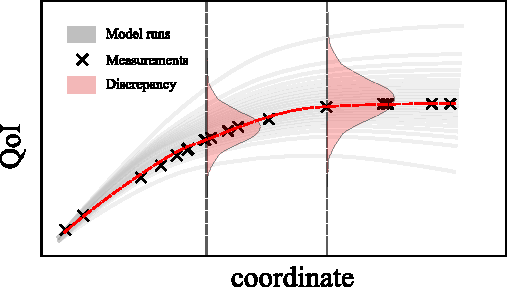
\includegraphics[scale=3]{figures/figure-likelihood.pdf}
\end{figure}
\end{columns}
 
\end{frame}
%===================================================================================================================
\begin{frame}
\begin{columns}
    \column{0.5\textwidth}
      \begin{figure} 
 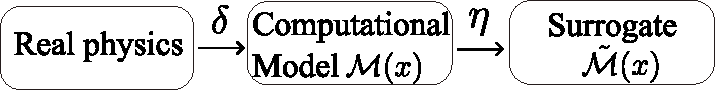
\includegraphics[scale=0.6]{figures/figure-TrunctionerrorandModeldiscrepancy.pdf}
\end{figure}
    \column{0.6\textwidth}
    \begin{block}{Other uncertainties?}
    \begin{itemize}
    \item Observation error $\boldsymbol{\varepsilon}$
    \item Model discrepancy $\delta(\boldsymbol{x})$
    \item Numerical/truncation error $\eta({\boldsymbol{x}})$
    \end{itemize}       
    \end{block} 
\end{columns}

\begin{block}{Revised:}
\begin{equation*}
\label{eq: COV_uncertainties}
\begin{aligned}
%https://rss.onlinelibrary.wiley.com/doi/abs/10.1111/1467-9868.00294
     \boldsymbol{y}
= &&
{\mathcal{M}}(\boldsymbol{x}) + {\delta(\boldsymbol{x})}
+ \boldsymbol{\varepsilon} \\
= &&
\tilde{\mathcal{M}}(\boldsymbol{x})
+ \eta({\boldsymbol{x}})
+ \delta(\boldsymbol{x})
+ \boldsymbol{\varepsilon}
\end{aligned}
\end{equation*}
\end{block}

\begin{alert}{Question: where should the uncertainties go to?}
\begin{equation*}               
\pi(\boldsymbol{x}|\mathcal{Y}) = 
\frac{{\textcolor{red}{\mathcal{L}(\boldsymbol{x}|\mathcal{Y})} \cdot \pi(\boldsymbol{x})}}{{\pi(\mathcal{Y})}}
= \frac{{\textcolor{red}{\mathcal{L}(\boldsymbol{x}|\mathcal{Y})} \cdot \pi(\boldsymbol{x})}}
{\int_{\mathcal{D}_{\boldsymbol{X}}} 
    \pi(\boldsymbol{x}) \pi(\mathcal{Y}|\boldsymbol{x}) {\rm{d}} \boldsymbol{x}}
\end{equation*}    
\end{alert}  
\end{frame}
%===================================================================================================================
%--------------------------------------------------------------------------------
\begin{frame}
\frametitle{Incorporating uncertainties into the $\mathcal{L}(\boldsymbol{x}|\mathcal{Y})$}
    

\begin{block}{If only consider observations error $\boldsymbol{\varepsilon}$}
\begin{equation*}
\boldsymbol{y}_i = \tilde{\mathcal{M}}(\boldsymbol{x})
+ \boldsymbol{\varepsilon}, i=1,\cdots,k; \ \boldsymbol{\varepsilon} \in \mathcal{N}(\boldsymbol{\varepsilon}|\boldsymbol{0},\boldsymbol{\Sigma})
\end{equation*}
\begin{equation*}        
        \label{eq: Likelihood function}
\begin{aligned}
 \mathcal{L}(\boldsymbol{x}|\mathcal{Y}) =& \prod_{i=1}^{k} N(\boldsymbol{y}_i|\tilde{\mathcal{M}}(\boldsymbol{x}),\boldsymbol{\Sigma}) \\
 =& \prod_{i=1}^{k}\frac{1}{\sqrt{(2 \pi)^{N}{\rm{det}} 
 (\boldsymbol{\Sigma})}}\exp\left(-\frac{1}{2}\left(\boldsymbol{y}_i - \tilde{\mathcal{M}}(\boldsymbol{x}\right)^{\mathsf{T}} \boldsymbol{\Sigma}^{-1}\left(\boldsymbol{y}_i - \tilde{\mathcal{M}}(\boldsymbol{x}\right)\right)
\end{aligned}
        \end{equation*}  
\end{block}

\begin{alertblock}{Incorporate all uncertainties into $\boldsymbol{\Sigma}$}
\begin{figure}[!ht]       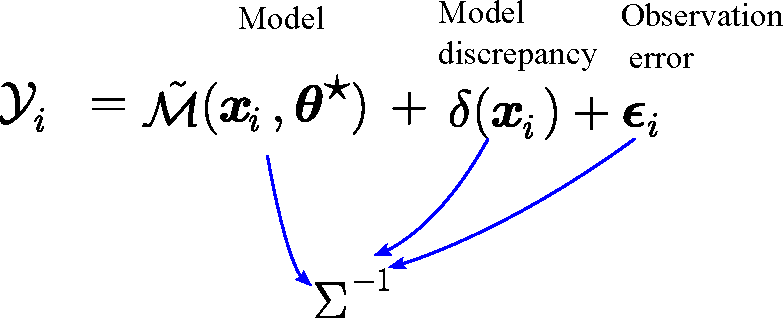
\includegraphics[scale=0.45]{figures/figure-CoVUncertainty.pdf}
\end{figure}
    
\end{alertblock}


\end{frame}
%--------------------------------------------------------------------------------
\begin{frame}
\frametitle{Bayesian inference results}
\begin{block}{Difficulty with calculating evidence $\pi(\mathcal{Y})$}
\begin{equation*}               
\textcolor{red}{\pi(\boldsymbol{x}|\mathcal{Y})} = 
\frac{{\mathcal{L}(\boldsymbol{x}|\mathcal{Y})} \cdot \pi(\boldsymbol{x})}{{\pi(\mathcal{Y})}}
\end{equation*}
\end{block}

% \textit{conjugate priors} examples: 
% \begin{itemize}
%     \item static Bayesian network
%     \item variant elimintion/ belief propagation
%     \item kalman filtering
% \end{itemize}

Computational methods:
 \begin{equation*}               \pi(\boldsymbol{x}|\mathcal{Y}) \approx 
{\mathcal{L}(\boldsymbol{x}|\mathcal{Y}) \cdot \pi(\boldsymbol{x})}
\end{equation*}     

Samples from the posterior can be obtained through \textit{Sampling methods} or \textit{Optimization methods}: \textit{MCMC}, \textit{variational methods},...
\end{frame}
%-------------------------------------------------------------------------------------------
